% 文档类采用pkuthss:http://www.ctan.org/pkg/pkuthss
% (需要其1.7.2或更早的版本,之后的版本将导致subfloat命令不可用)

% 在macOS上编译时,指定字符集为mac(覆盖掉ctexopts.cfg中的配置):
%\documentclass[UTF8, fontset = mac]{pkuthss}
\documentclass[UTF8]{pkuthss}

% 参考文献所需的包和自定义命令
\usepackage{cite}
\newcommand{\supercite}[1]{$^{\mbox{\scriptsize \cite{#1}}}$}
\newcommand{\wuhao}{\fontsize{10.5pt}{10.5pt}\selectfont}    % 五号, 单倍行距

% 表格所需的包和自定义命令
\usepackage{makecell}
\usepackage{multirow}
\usepackage{colortbl}
% 使用&\tabincell{c}{}&可在单元格中自动换行
\newcommand{\tabincell}[2]{\begin{tabular}{@{}#1@{}}#2\end{tabular}}

% 算法伪码所需的包
\usepackage{algorithm}
\usepackage{algorithmic}

% 让脚注编号每页都从1开始。
\usepackage[perpage]{footmisc}

% 设定文档的基本信息。
\pkuthssinfo{
	cthesisname = {博士研究生学位论文}, ethesisname = {Doctor Thesis},
	ctitle = {自适应视频流媒体中的关键技术研究}, etitle = {Research on Key Technologies of Adaptive Video Streaming},
	cauthor = {孟胜彬},
	eauthor = {Shengbin Meng},
	studentid = {1101111141},
	date = {二〇一六年五月},
	school = {信息科学技术学院},
	cmajor = {计算机应用技术}, emajor = {Computer Science},
	direction = {数字视频信息处理},
	cmentor = {郭宗明\ 研究员}, ementor = {Prof.\ Zongming Guo},
	ckeywords = {视频流媒体,码流截取,码率自适应,视频直播}, ekeywords = {Video streaming, Bitstream extraction, Rate adaptation, Live streaming}
}

\begin{document}
	% 以下为正文之前的部分,默认不进行章节编号。
	\frontmatter
	% 此后到下一 \pagestyle 命令之前不排版页眉或页脚。
	\pagestyle{empty}
	% 自动生成封面。
	\maketitle
	% 封面要求单面打印,故需新开右页。
	\cleardoublepage

	% 版权声明。
	\chapter*{版权声明}
\thispagestyle{empty}

任何收存和保管本论文各种版本的单位和个人,
未经本论文作者同意,不得将本论文转借他人,
亦不得随意复制、抄录、拍照或以任何方式传播。
否则一旦引起有碍作者著作权之问题,将可能承担法律责任。

% 若需排版二维码,请将二维码图片重命名为“barcode”,
% 转为合适的图片格式,并放在当前目录下,然后去掉下面 3 行的注释。
%\vfill\noindent
%\includegraphics[height = 5em]{barcode}


	\cleardoublepage

	% 此后到下一 \pagestyle 命令之前正常排版页眉和页脚。
	\pagestyle{plain}
	% 重置页码计数器,用大写罗马数字排版此部分页码。
	\setcounter{page}{0}
	\pagenumbering{Roman}

	% 中英文摘要。
	\begin{cabstract}
近年来,计算机技术的发展使得移动设备逐渐普及,通信技术的发展使得互联网无处不在。在这样的条件下,通过网络随时随地观看视频成为可能,而且逐渐发展为视频内容消费的主要形式。这种无需先下载好全部视频数据而是一边下载一边播放的技术称为视频流媒体。视频流媒体的相关应用,如按需点播、实时直播、在线教育、视频会议等,已经成为人们生活中不可或缺的部分。在这前所未有的机遇同时,视频流媒体也面临着网络异构性和带宽波动的挑战。为应对这一挑战,视频流媒体系统需要能够根据不同的网络条件自动调整所发送的数据码率,以适应带宽的变化。本文\footnote{本研究得到国家自然科学基金(项目编号61271020)和国家科技支撑计划(项目编号2014BAK10B02) 资助。}从数据源和数据传输两方面入手,结合点播和直播两种应用模式,对自适应视频流媒体中的关键技术进行了较为全面深入的研究。首先,本文针对可伸缩视频数据源提出了新的失真模型和码流截取方案,在支持可变码率的同时提供尽可能高的视频质量;其次,本文为视频点播系统设计了新的码率自动调整策略,用控制论的方法来解决如何适应带宽变化的问题;最后,本文详细分析了现在非常流行的视频直播系统的传输过程,结合直播的特点提出了数据上传时的码率自适应算法。本文主要的创新性贡献可以归纳为如下三个部分:
\begin{enumerate}
\item {采用线性误差模型的可伸缩视频码流截取方案}\\
对于可伸缩视频数据源,本文首先推导并验证了一个线性误差模型,用于准确估计丢弃任意数据包组合带来的失真变化;然后采用该模型设计了一个贪心型算法来根据每个数据包的码率和失真影响对其赋优先级,作为截取子流时丢弃数据包的顺序。相比于参考软件,这一码流截取方案能够在同样的复杂度和码率限制下取得更高的视频质量。
\item {基于PID控制思想的点播系统码率自适应算法}\\
本文基于经典的比例-积分-微分(PID)控制思想,为视频点播系统的数据传输过程提出了一个综合考虑带宽的历史状况、当前状态和未来趋势的码率自适应算法,既能充分利用带宽,传输较高的视频质量,又能减小带宽波动的影响,保证视频质量的平滑性。该算法集成在了苹果公司QuickTime流媒体服务器的开源版本上,将发送的视频平均质量提高了8.6\%,质量波动降低了24.8\%。
\item {基于缓冲区分析的直播系统码率自适应算法}\\
为给视频直播中的数据上传阶段增加码率自适应的特性,本文首先详细分析了系统整个传输过程中各个缓冲区的关系,建立了一个多缓冲区模型;然后把上述点播系统中用到的PID方法与多缓冲区模型相结合,提出了一个有效的上传过程码率自适应算法。相比于没有自适应的上传过程,带宽的利用率得到了提升,视频播放的连续性也得到了改善。
\end{enumerate}
\end{cabstract}

\begin{eabstract}
In recent years, the development of computer technology has made the mobile devices popular, and the communication technology has made the Internet accessible everywhere. Under such circumstances, watching videos at any time and any place becomes possible, and even an increasingly important way for people to consume video content. This is called video streaming, where the video can play as the data are being transmitted, before the entire file has been downloaded. Applications of video streaming, e.g., video on demand (VoD), live broadcasting, online education, and remote video conference, have become an indispensable part of people's life. Along with those opportunities, video streaming also has the big challenge brought about by the variety of networks. To cope with this challenge, the video streaming system should be able to adjust the video's bitrate or quality according to the network condition. In other words, the video streaming system needs to be adaptive. In this paper, we investigate and solve the key problems in adaptive video streaming. First, focusing on the adaptive video streaming system based on the Scalable Video Coding (SVC) extension of the H.264/AVC video coding standard, this paper proposes a novel bitstream extraction scheme to provide highest possible video quality while supporting bitrate adjustment at the same time. Second, this paper designs a new rate adaptation algorithm for the VoD system, adjusting the bitrate to fit the current bandwidth from the control perspective. And finally, this paper analizes the transmission process of live video streaming in detail and proposes a rate adaptation algorithm for its uploading stage. The innovative contributions of this paper can be summarized as follows.
\begin{enumerate}
\item {Bitstream extraction scheme utilizing a linear error model}\\
For scalable video data source, a simple and effective linear error model is proposed and verified, which can be used to accurately estimate the distortion caused by discarding any combination of data packets from an SVC bitstream. Then utilizing this model, a greedy-like algorithm is designed to assign priority for each data packet according to its Rate-Distortion (R-D) impact, thus enabling optimized bitstream extraction. Comparing with the reference software, this extraction scheme achieves higher video quality with the same computational complexity and bitrate constraint.
\item {Rate adaptation algorithm for VoD systems based on the idea of PID control}\\
Based on the classical Proportional-Integral-Derivative (PID) controller, a rate adaptation algorithm is proposed for the data transmission process of VoD systems. By monitoring and predicting past, current and future bandwidth information, the algorithm is able to reduce quality fluctuation while still preserving a high quality level. Integrated into the open source version of Apple's QuickTime streaming server, this algorithm increases the streamed video's quality by 8.6\% and decreases the quality variance by 24.8\% at the same time.
\item {Rate adaptation algorithm for live streaming systems based on analysis of data buffers}\\
This paper also proposes to add adaptation for the data uploading stage of live video streaming systems. A multi-buffer model is built based on analysis of the several data buffers during the transmission, and it is combined with the PID method to provide rate adaptation effectively. Compared with non-adaptive uploading, the bandwidth utilization is increased and the playback continuity is improved.
\end{enumerate}
\end{eabstract}
	% 自动生成目录。
	\tableofcontents
	\listoffigures
	\listoftables

	% 以下为正文部分,默认要进行章节编号。
	\mainmatter
	% 各个章节
	\chapter{绪论}

\section{研究背景和意义}

进入二十一世纪以来,人们表示和传递信息的媒介从文本、声音扩展到了图像、视频。如今视频已经成为人们生产和生活中不可缺少的部分。另一方面,在计算机技术和通信技术的推动下,人们对网络的依赖和要求也越来越高。
智能手机、平板电脑等移动设备的普及,Wi-Fi、4G等无线网络的覆盖,让人们能够随时随地访问互联网。这样的环境催生并促进了一项技术的蓬勃发展,这就是视频流媒体。

视频流媒体简单来说就是通过网络在线播放视频。所谓流媒体,是指音视频等多媒体数据通过网络以连续稳定的流的形式传输到客户端的一系列技术、协议和方法的总称。在视频流媒体中,视频数据从服务器连续不断地传输到客户端,客户端可以一边接收一边播放,无需等待整个文件发送完毕。与下载方式相比,这种采用流式传输的视频播放具有显著的优点\supercite{Li2002},包括:1)启动延迟大大缩短,用户可以在等待几秒或十几秒的缓冲后就立即开始观看;2)视频数据不在客户端长时间驻留,不仅节省了用户存储空间,也一定程度上避免了内容版权保护问题;3)支持数据的实时生成和获取,大大扩展了视频应用场景的范围。正是由于其优秀的特性,视频流媒体得到了广泛的应用,逐渐成为人们消费视频内容的主要形式\supercite{Chen2013}。

视频流媒体应用按照其对实时性要求的不同可以分为点播和直播两大类。在点播应用中,内容提供商将预先制作好的视频放在服务器上,并发布内容的描述信息和链接,用户选择自己感兴趣的内容请求播放相应的视频。典型的例子是在线视频网站,如国外的YouTube\footnote{https://www.youtube.com/}、Netflix\footnote{https://www.netflix.com/},国内的优酷\footnote{http://www.youku.com/}、乐视\footnote{http://www.le.com/}等。大多在线教育网站如Coursera\footnote{https://www.coursera.org/}、网易公开课\footnote{http://open.163.com/}等也属于视频点播类应用。在直播应用中,视频数据则是通过现场录制实时生成的,上传到流媒体服务器之后再即时分发给观看者,具有很强的时效性。这类应用包括现在互联网上正兴起的秀场、游戏、生活类直播软件,以及已经很成熟的远程监控、视频会议等等。直播应用往往也会把实时事件的内容存储起来,后续以点播的形式继续提供。

网络条件的改善,采集与播放设备的普及,使得视频流媒体应用进入了一个高速增长的时期。根据Cisco的一项预测\footnote{http://www.cisco.com/c/en/us/solutions/collateral/service-provider/ip-ngn-ip-next-generation-network/white\_paper\_c11-481360.html},从2014年到2019年,视频流量在所有互联网流量中的占比将从64\%上升至80\%。路透社的一篇报道\footnote{http://www.reuters.com/article/us-internet-consumers-cisco-systems-idUSKBN0EL15E20140610}指出,在美国这一比例在2018年即将达到83\%。可见,视频流媒体正迎来一个高峰期。

在前所未有的机遇同时,视频流媒体也面临着诸多挑战。一方面,网络状况变得越来越复杂,传输可用带宽不可预知,如何保证视频数据及时高效地发送给每个用户成为了一个需要考虑的问题。另一方面,大部分用户终端设备的计算能力还很低,而视频分辨率在不断增大,且编解码的复杂度也越来越高,用户收到视频数据后的解码和显示所需计算量越来越大,快速实时解码变得越来越困难。下面对这两大挑战进行具体说明。

首先,从网络状况来看,目前既有几百kb/s速度的拨号或3G上网,又有几十Mb/s速度的局域网或光纤接入,而且随着移动通信网与Internet的融合,无线与有线网络混联,使得带宽和信道质量更加不确定。在这样异构且波动的网络环境下,确定的视频流很难高效传输,也很难满足不同接入用户的需求。举例来说,如果设置一个较低的码率,则对应的视频质量不高,达不到带宽充足用户的满意度;而如果设置较高的码率,则对低带宽的用户或者在带宽波动较大的情况下,会导致视频无法流畅播放,带来不好的用户体验。即使是同一个用户,由于其所在网络环境会不时变化,如果视频数据以恒定的速率传输,观看体验几乎不可能达到最优。

其次,从用户终端来看,虽然前沿处理器计算能力不断在增强,但大部分用户的设备用的还是几年前的处理器,运算能力相当有限。尤其是对于智能手机和平板电脑而言,由于电池的制约,只能采用ARM架构的低功耗处理器。与此截然相反的是,现在的采集和显示设备像素成倍增加,视频分辨率早已突破了720p(1280x720)乃至1080p(1920x1080)的限制,向4K(3840x2160)发展。为了压缩这些高清和超高清的视频,视频编码的技术复杂度也越来越高。高分辨率的视频和高复杂度的编码技术,使得解码计算量大大增加。在通用处理器上的实时解码,成为了限制视频流媒体服务进一步改善的瓶颈。

考虑到视频流媒体的广泛应用,如何解决这些问题从而进一步改善流媒体服务质量,具有重要的现实意义。视频流媒体的研究既受到了工业界的关注,也成为了学术界的一大热点。

\section{研究框架和问题}

视频流媒体是视频与流媒体的结合,这个领域的研究也涉及包括编码和传输在内的多个子领域。视频流媒体的研究可以从系统模块的角度分为以下几个部分(参见图\ref{fig:research-framework}):

\begin{itemize}
	\item 数据源端的研究,一方面是进行高效的压缩编码,以尽可能少的数据表示尽可能高的视频质量;另一方面是提供具备灵活性的码流,支持码率的变化甚至考虑容错,等等。
	\item 传输过程的研究,即如何又快又好地将视频数据送给用户,包括改善网络状况以提高传输的吞吐量和可靠性,合理公平地利用带宽资源,根据带宽情况自适应地调整传输速率等。
	\item 客户终端的研究,即优化用户设备收到视频码流之后的播放阶段,包括如何快速解码,进行一些画质增强等后处理过程从而更好地显示,等等。
\end{itemize}

\begin{figure}[h]
	\centering
	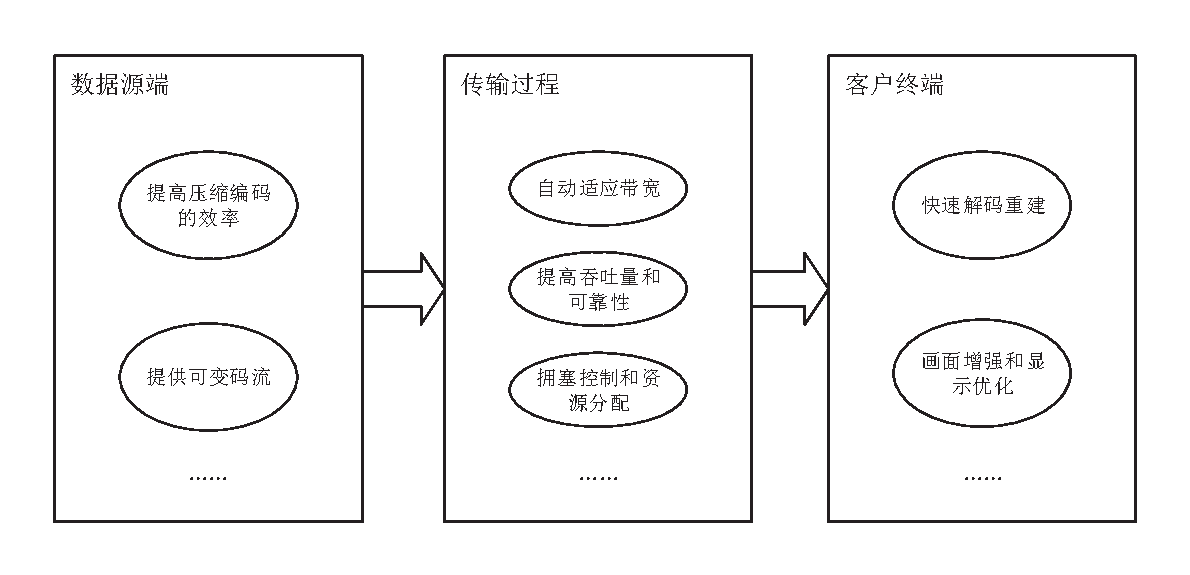
\includegraphics[width = 1.0\linewidth]{eps/research-framework}
	\caption{视频流媒体研究框架 \label{fig:research-framework}}
\end{figure}

数据源端对视频码流可变性的支持,再加上传输中自动调整码率以适应带宽的变化,结果就是所谓的自适应视频流媒体。在自适应视频流媒体中,服务器发送给客户端的视频流的码率能自动根据带宽的变化情况进行调整。这一特性能够很好地应对上一节中提到的网络异构和带宽波动带来的挑战。虽然其他方面的研究,例如对编码效率的提升、对网络架构和协议的改进,也非常重要,但本文主要关注的是自适应视频流媒体相关技术的研究。

通常有两种选择可以用来实现自适应视频流媒体。第一种选择是采取多码流的方法。多码流方法的原理很简单,就是预先编好不同码率的多个码流存放在服务器上,根据网络情况选取其中合适的一个进行传送。近年来兴起的HTTP动态自适应流媒体(Dynamic Adaptive Streaming over HTTP,  DASH)\supercite{Sodagar2011}就属于这类方法。如图\ref{fig:DASH}所示,DASH系统在服务器端提供不同码率的多个码流切片,客户端通过HTTP协议拉取数据,在某个时间段内可以选择性地接收这几个码流中任何一个的切片,通过在多码流之间切换来动态适应带宽波动。第二种选择是采用可伸缩视频编码\supercite{SVC-Overview}技术。作为国际视频编码H.264/AVC\supercite{H.264}的扩展之一,可伸缩视频编码目的就是在单个码流中加入伸缩性的支持,使其码率能够根据需要改变。因此,用它来实现自适应视频流媒体系统正符合其设计初衷。

\begin{figure}[t]
	\centering
	\includegraphics[width = 1.0\linewidth]{eps/DASH}
	\caption{DASH系统的工作原理示意图\label{fig:DASH}}
\end{figure}

多码流联播方案的优点是无需对已有的程序和系统做较大的改动,因此比较易于部署\supercite{Bouten2014}。很多商业视频网站(如YouTube、优酷等)已经用它实现了自适应功能。但是,多码流方案能提供的适应范围和粒度非常有限。例如,YouTube最多只提供240p、360p、480p、720p和1080p这五个等级,而优酷只提供标清、高清、超清这三个画质(参见图\ref{fig:13})。此外,多个码流的编码和存储需要大量的计算资源和磁盘空间,使得时间和空间开销成倍增加。要想以合理的代价提供精细无缝的自适应性,就需要采用可伸缩视频编码的方案。可伸缩视频码流能够以非常小的数据粒度进行码率调整,而且性能分析表明可伸缩视频编码的压缩效率远高于同一内容多次编码的多码流方法\supercite{SVC-Performance}。正是因为这些优势,采用可伸缩视频编码来实现自适应视频流媒体从技术上来说是一个更好的方案,也吸引了学术界很多研究者的关注\supercite{Chuah2012, Zhu2013, Dan2013, Yang2014, Cicalo2014}。

\begin{figure}[t]
	\centering
	\includegraphics[width = 1.0\linewidth]{clip/13.png}
	\caption{优酷网视频码率自适应功能图示\label{fig:13}}
\end{figure}

从图\ref{fig:research-framework}所示的研究框架中可以看出,采用可伸缩视频编码或是采用DASH之类的多码流方案,其区别只在于数据源端提供灵活码流的方式不同。可伸缩视频作为数据源时,在给定码率下如何最优地从整个码流中截取出一个子流用于发送是需要研究的问题之一,DASH系统则不存在这个问题。而对于在传输中如何自动调整码率以适应带宽的变化,却是二者共有的问题。此外,无论是何种视频流媒体系统,当用户设备收到视频流后都需要进行解码和播放。为了在计算资源有限的设备上满足实时播放的要求,通用处理器上的解码优化也是值得重视的问题之一。这些问题的解决,是提高视频流媒体服务质量和用户体验的关键。

\section{本文研究内容和主要贡献}

本文结合视频流媒体所面临的挑战,对上面提到的关键问题进行研究。首先,本文针对可伸缩视频数据源提出了新的失真模型和码流截取方案,在支持可变码率的同时提供尽可能高的视频质量;其次,本文为视频数据的传输过程设计了新的码率自动调整策略,用控制论的方法来解决适应带宽变化的问题;最后,为了保证用户终端收到码流后能够快速实时的解码并播放,本文研究了新一代国际视频编码标准HEVC(High Efficiency Video Coding)\supercite{HEVC-Overview}的解码过程,提出了新的优化算法来对其进行加速。本文主要的创新性贡献可以归纳为如下三个部分:
\begin{enumerate}
\item {采用线性误差模型的码流截取方案}\\
作为码率适应带宽波动的前提条件,视频流媒体中的数据源需要能够灵活调整。可伸缩视频编码将数据划分为基本层和增强层,通过丢弃增强层的数据包来实现即时码率变化。从完整的可伸缩码流中丢弃部分数据得到一个子流的过程称为码流截取。本文以最小化特定截取码率限制下的视频失真为目标,首先提出了一个线性误差模型来估计丢弃任意数据包组合带来的失真变化,然后利用它设计了一个贪心型算法来根据每个数据包的码率和失真影响对其赋优先级,作为截取过程中丢包的顺序。相比于参考软件,这一码流截取方案能够以更低的复杂度取得更高的视频质量。
\item {基于PID控制思想的码率自适应算法}\\
自适应流媒体的另一个关键问题是传输过程中的码率调整策略,即在可用带宽不断变化的情况下,决定何时调整码率并确定调整到多少。本文基于经典的比例-积分-微分(Proportional-Integral-Derivative,PID)控制思想,提出了一个综合考虑带宽的历史状况、当前状态和未来趋势的码率自适应算法,既能充分利用带宽,传输较高的视频质量,又能减小带宽波动的影响,保证视频质量的平滑性。该算法在点播和直播的实际测试中都表现出了很好的性能,而且很容易扩展到各种自适应流媒体系统。
\item {高度优化的HEVC解码器设计与实现}\\
视频流媒体的最后一个阶段是码流在用户终端设备上的解码播放。为此,本文设计并实现了一个高度优化的HEVC软件解码器,将数据级和任务级并行方法相结合,显著提高了各个解码模块的计算效率以及整体解码速度。该解码器分别在主流的桌面和移动处理器上达到了4K ($3840 \times 2160$) 和720p ($1280 \times 720$) 视频的实时解码要求,并已成功应用于业界知名的视频流媒体平台迅雷看看,为进一步改善用户在线观看视频的体验提供了技术支撑。
\end{enumerate}

\section{本文的结构安排}

本文共分为六章,后续章节具体内容安排如下。

第二章概述视频流媒体领域的研究基础和相关工作。首先对视频编码和流式传输的基础知识进行简要介绍,为后文内容做准备;然后结合本文的研究内容对码流截取、码率自适应、解码器优化这几个问题和已有工作进行分析。

第三章讨论采用线性误差模型的码流截取方案。首先针对可伸缩视频推导并验证线性误差模型,然后介绍采用该模型的失真估计方法和以码率失真影响为度量标准的优先级赋值算法。最后展现并分析所提出的码流截取方案的实验结果。

第四章讨论基于PID控制思想的码率自适应算法。首先对PID控制器做简单的介绍,然后将PID模型运用到视频传输中的码率自适应问题,提出了一个新颖的码率自适应算法。该算法被集成在了实际点播和直播流媒体系统中,其有效性通过对比实验得到了验证。

第五章讨论针对新一代视频编码标准HEVC的解码优化工作。以重新设计的解码器原型为基础,首先采用单指令多数据技术对特定解码模块进行加速,然后引入帧级并行解码框架提高了在多核处理器上进行多线程解码的速度,最后对上述方法所取得的优化效果进行了评测。

第六章总结全文内容并对未来工作和应用前景进行展望。
	\chapter{研究现状和相关工作}
本章介绍研究现状和相关工作。

\section{流媒体研究领域综述}

\section{视频编解码相关工作}

\section{SVC码流截取的相关工作}

\section{码率自适应的相关工作}
	\chapter{基于线性误差模型的码流截取}
本章介绍码流截取算法。

\section{问题描述}

\section{线性误差模型}

\subsection{模型推导}

\subsection{误差向量获取}

\subsection{模型验证}

\section{数据包优先级赋值}

\subsection{优先级度量标准}

\subsection{贪心法赋值}

\subsection{无参考源的情况}

\section{实验结果}

	\chapter{基于PID控制器的码率自适应算法}

\section{引言}

在实际网络条件下,带宽波动是不可避免的。对于一个视频流媒体系统而言,能够根据带宽变化来自适应地调整发送码率能为用户提供更好的服务。在上一章中,我们通过可伸缩视频的码流截取,使得码率能够调整;在本章中,我们主要关注如何调整。由于视频码率与视频质量一般来说是正相关的,调整码率也就是调整所传送视频的质量。因此,本章解决的问题又被称为质量控制问题。我们将基于经典控制实践中的PID思想,设计一个综合考虑带宽的历史状况、当前状态和未来趋势的码率自适应算法,从而提高发送视频的总体质量和平滑性。

\section{PID控制器简介}

PID控制器\footnote{http://en.wikipedia.org/wiki/PID\_controller}是一个在工业控制系统中常用的闭环反馈控制器。PID控制中的两个重要概念是过程变量和控制目标。过程变量代表着系统当前的状态,而控制目标是系统希望达到的理想状态。PID控制的基本思想就是根据过程变量和控制目标之间的误差来确定一个控制输出,该输出反馈作用到系统以最小化上述误差。

PID控制器的控制输出一般如下定义:
\begin{equation}
\label{eq:pid-output}
u(t) = {K_p} \cdot e(t) + {K_i} \cdot \int_0^t {e(\tau )d\tau }  + {K_d} \cdot \frac{d}{{dt}}e(t) \: ,
\end{equation}
其中$e(t)$指代过程变量与控制目标在时刻$t$的误差,$K_p$、$K_i$、$K_d$是三个可调参数,依次称为比例增益、积分增益和微分增益。公式(\ref{eq:pid-output})的结果通过某种方式来影响系统状态,使得过程变量朝着控制目标变化。

作为一个灵活有效的控制技术,PID可以被用来解决各种各样的控制问题\supercite{Wong2004}\supercite{Li1999}。在本文的工作中,我们基于它设计了一个码率自适应算法,用来控制视频流媒体中的视频质量。

\section{基于PID的码率自适应}

本节首先介绍质量等级的概念,来将视频流媒体中的视频质量和码率值离散化,接着定义在所提出的码率自适应算法中用到的过程变量及其控制目标。之后,我们详细解释控制模型和自适应算法细节,并简要讨论一下模型参数的选取和调优。

\subsection{质量等级划分}

视频质量或码率是一个连续的值,以任意的精度来控制或调整它是不现实的。因此,我们首先提出一个质量层级的概念来离散化视频质量和码率。当需要调整时,我们只是增加或减少质量等级。每一个质量等级对应一个确定的码率。高等级对应高码率,反之亦然。有多少个质量等级以及它们跟具体码率值如何对应可以根据实际需求来确定。质量等级越多,系统就能越精细地调整码率来适应带宽变化。如绪论中所说,用多码流实现的自适应流媒体系统只能提供有限的几个质量等级,而基于可伸缩视频编码的流媒体系统能够以更高的精度来定义质量等级。

\subsection{过程变量和控制目标}

在本文所提出的质量控制算法中,所选取的过程变量称为“实际与检测间隔比”。下面介绍其具体定义。

\begin{figure}[h]
	\centering
	\includegraphics[width = 0.9\linewidth]{figures/Intervals.png}
	\caption{达尔文流媒体服务器中的两个时间线 \label{fig:intervals}}
\end{figure}

在达尔文流媒体服务器中,有两个时间线非常重要。第一个是推送时间线(push time),也就是视频数据包被推送到缓冲区的时间;第二个是播放时间线(play time),也就是数据包应该在播放中被显示的时间(通常记作该数据包的PTS)。这两个时间线的关系如图\ref{fig:intervals}所示。服务器程序会定时检测这两个时间线,并根据数据包的延迟来决定是否需要调整发送的视频质量。图\ref{fig:intervals}中的两个间隔,即检测间隔(check interval)和实际间隔(actual interval),值得我们注意。在理想情况下,每次检测间隔中服务器推送的数据量应该恰好能实际播放等于检测间隔的一段时间,也就是\textit{actual\_interval} = \textit{check\_interval}。如果实际间隔小于检测间隔,说明这段时间内推送了较少的数据,推送数据变慢很可能是带宽有所下降。反过来,如果实际间隔大于检测间隔,说明这段时间内推送了较多的数据,意味着网络条件良好且数据被快速推向客户端。这两个间隔的比值,也就是所谓的“实际与检测间隔比”,能够反映当前推送的速率是否与网络带宽相符。

“实际与检测间隔比”适合用作质量控制有三方面的原因。第一,这个比例直接对应着适合带宽的码率与当前传输的码率的比值,只需据此进行调整就可以准确地使码率符合带宽。第二,根据定义这个比例的理想值就是1,这就是算法的控制目标,无需再通过别的方法确定。第三,这个值在实际系统中便于计算,普适性较好。

\subsection{控制模型}

在通常的PID控制器中,控制输出是用过程变量与控制目标之间的差值进行比例、积分、微分求取出来的。考虑到我们所选的过程变量是一个比例,且控制目标是1,本文对通常的PID控制器做了修改,提出了一个基于比例的模型。在这个模型中,过程变量直接被用来计算控制器输出,而且所有求差的运算都被适当的改为了求比例的运算,以保持模型的合理正确性,如下所示:

\begin{equation}
\label{eq:ut}
{u_t} = {K_p} \cdot E_p^t + {K_i} \cdot E_i^t + {K_d} \cdot E_d^t ,
\end{equation}

\begin{equation}
\label{eq:ep}
E_p^t = \frac{{actual\_interva{l_t}}}{{check\_interva{l_t}}} ,
\end{equation}

\begin{equation}
\label{eq:ei}
E_i^t = \frac{{long\_actual\_interva{l_t}}}{{long\_check\_interva{l_t}}} ,
\end{equation}

\begin{equation}
\label{eq:ed}
E_d^t = E_p^t/E_p^{t - 1} ,
\end{equation}

\begin{equation}
\label{eq:long-actual}
long\_actual\_interva{l_t} = \sum\limits_{\tau = {T_l}}^t {actual\_interva{l_\tau}} ,
\end{equation}

\begin{equation}
\label{eq:long-check}
long\_check\_interva{l_t} = \sum\limits_{\tau = {T_l}}^t {check\_interva{l_\tau}} .
\end{equation}

在公式(\ref{eq:ut})中:$K_p$、$K_i$、$K_d$分别表示比例部分、积分部分、微分部分的可调参数;$E_p^t$、$E_i^t$、$E_d^t$则对应各部分在第t次检测时的值,它们的定义如公式(\ref{eq:ep})至(\ref{eq:long-check})所示;控制器输出$u_t$将用来计算适合当前带宽的码率,并据此选择要传送的质量等级。

在公式(\ref{eq:long-actual})和(\ref{eq:long-check})中,$T_l$代表上一次质量等级改变的时间。按照理论定义,积分部分应该从系统启动开始记录,但在实际环境中,网络带宽有可能变动非常大,如果积分部分记录累积太长时间将不适合反映当前的网络条件,从而减缓调整质量的决策。因此这里采用了一个折衷,选择从上一次质量等级变化的时间开始计算积分部分。

这个基于比例的模型对于所选的过程变量和控制目标比通用模型更加简单有效。而且,在该模型中,当三个参数进行归一化处理后,控制器输出具备明显直观的意义。从公式(\ref{eq:ep})至(\ref{eq:long-check})容易看出,$E_p^t$、$E_i^t$、$E_d^t$这三个值都是在1附近波动的比值;而根据公式(\ref{eq:ut}),控制器输出$u_t$可以被视作这三个比值的加权平均(三个参数作为权值)。因此,$u_t$也是一个在1附近的比值,它对应着适合当前带宽的码率与当前发送码率的关系。换句话说,如果$u_t$大于1,那么控制器决定当前发送码率需要增加;反之,如果$u_t$小于1,意味着控制器认为当前发送码率需要减小。用$u_t$作为一个乘子来调整当前发送的码率,我们就能控制流媒体系统符合带宽的变化。

\subsection{自适应算法}

综上,本文提出的码率自适应算法描述如下:

\begin{algorithm}
	\caption{基于PID的码率自适应算法}
	\label{algo:control}
	\begin{algorithmic}
		\STATE 准备发送数据包
		\STATE check\_interval = curr\_time -- last\_check\_time
		\STATE actual\_interval = curr\_media\_time -- last\_check\_media\_time
		\STATE long\_check\_interval += check\_interval
		\STATE long\_actual\_interval += actual\_interval
		\STATE 根据公式(\ref{eq:ep}) - (\ref{eq:ed})计算$E_p^t$、$E_i^t$、$E_d^t$的值
		\STATE output = ${K_p} \cdot E_p^t + {K_i} \cdot E_i^t + {K_d} \cdot E_d^t$
		\STATE new\_bitrate = output * curr\_bitrate
		\STATE new\_level = get\_level(new\_bitrate, bitrate\_of\_level[])
		\IF {质量等级变化}
		\STATE long\_check\_interval = 0
		\STATE long\_actual\_interval = 0
		\STATE curr\_bitrate = bitrate\_of\_level[new\_level]
		\ENDIF
		\STATE 根据新的质量等级发送数据包
	\end{algorithmic}
\end{algorithm}

相比于其他的调度策略,这个基于PID的自适应算法具有以下几个优点。首先,该算法不仅仅依据当前状态或者固定时间点的信息来做决策,因此质量调整可以在任何合适的时间发生。其次,因为PID模型(微分部分)在某种程度上考虑了对未来的预测,该算法能够判断带宽在未来一段时间内是否会变得足够大或足够小,因此能避免一些不必要的调整。最后,该算法并不一定一次只调整一个质量等级,这就使得当带宽剧烈下降时能够快速下调质量以保证流畅播放,而当系统启动时能够快速上调质量以使用户尽早收到更清晰的视频。

\subsection{参数选取与调优}

与工业界的其他PID控制系统一样,本文提出的算法中三个参数的选取也是跟实现相关的。大多数情况下,为取得最优的效果,需要手动试错调节。每个参数对系统的不同方面产生影响,知道这些影响有助于进行参数选取。一般来说,PID控制器中的比例部分会影响系统的稳定性。如果比例增益$K_p$过高,系统容易变得不稳定。但是,太低的$K_p$又会导致过长的上升时间,使系统响应迟缓。积分部分除了能消除稳态误差,还能加速过程变量向控制目标的变化。这意味着,增大$K_i$能减小上升时间,提高系统的响应速度。但是,积分部分会累积过去一段时间的误差,使过程变量容易超出目标值(即超调),因此过大的$K_i$也会导致系统不稳定。上述这些隐患都能通过微分部分来校正。微分部分通过预测系统行为,具有减小超调、提高稳定性的双重效果。但是微分部分的特点是对误差分成敏感,也正是因为此,工业实践中微分增益$K_d$通常都设置的比较低。

本文采用了经典的Ziegler--Nichols方法\supercite{Ziegler1942}来进行参数选取。该方法首先把积分和微分参数设为0,调节比例参数$K_p$到系统开始震荡时的值$K_u$,假设震荡周期为$T_u$,那么设置$K_p = 0.6K_u$、$K_i = 2K_u/T_u$、$K_d = K_u \cdot T_u/8$。再将$K_p$、$K_i$和$K_d$进行归一化,就得到最终的参数:$K_p = 0.22$,$K_i = 0.73$,$K_d = 0.05$。

\section{实验结果}

\section{本章小结}
	\chapter{基于缓冲区分析的直播系统码率自适应算法}

在上一章中,我们以达尔文流媒体服务器作为平台为视频点播系统的传输过程设计了一个码率自适应算法。本章针对如今越来越流行的用户生成内容(User Generated Content, UGC)直播应用进行研究,提出了一个基于传输中缓冲区分析的码率自适应算法,来改善从数据产生设备向服务器上传数据的效率。

\section{视频直播系统概述}

在有些视频直播系统中,视频内容由服务器或者与服务器通过局域网紧密连接的设备生成。在这种情形下,视频直播和视频点播系统有很大的相似性。这时视频数据的传输主要是从服务器到观看者客户端。直播服务器将动态生成的视频数据发送给客户端,和点播最主要的区别在于传输速率不能超过视频数据生成的速率,因为当所有生成的数据都传输之后,客户端需要等待下一个数据片段就绪\supercite{Thang2014}。

但在UGC直播模式下,服务器本身不充当初始的内容产生方, 而是在其他设备上持续生成的视频内容经过互联网(具有不确定的带宽和不可忽略的延迟)传输到中转服务器,然后再由服务器分发给观看者。目前这种模式的直播越来越流行,因为已经非常普及的智能手机成为了理想的内容产生方和观看接收方。图\ref{fig:07}展示了通用的手机视频直播系统的主要模块。集成了高效视频编码器的智能手机作为内容提供者,将实时视频数据传输到服务器。服务器所在的本地网络内设有转码器和提供播放服务的内容服务器。转码服务器会将上传的码流实时转码成多路具有不同码率的视频流,交由内容服务器供不同的观看者播放。播放客户端可以根据自己的网络环境选择最合适的码率,从服务器获取视频数据。

\begin{figure}[t]
	\vspace{10pt}
	\vspace{10pt}
	\centering
	\includegraphics[width = 1.0\linewidth]{clip/07.png}
	\vspace{10pt}
	\caption{通用的手机直播系统模型\label{fig:07}}
	\vspace{10pt}
\end{figure}

容易看出,在这样的直播系统中,依次有两个传输阶段。第一个是上传阶段,即内容产生方将录制的视频传给服务器;第二个是分发阶段,即视频数据发送给观看者。第二个阶段与点播系统类似,而且服务器端转码成多码流正是为了提供这一阶段传输的码率自适应性。本文主要关注的是第一个阶段,即上传阶段的码率自适应问题。

为了提供高质量的直播视频流,内容产生方理论上应该上传尽可能高码率的视频。然而高码率可能导致数据传输时间过长,造成接收端的播放中断。因此,在带宽变化的情况下,而内容产生方一方面需要尽可能利用网络吞吐量传输高质量的视频,另一方面还要保证接收端的流畅播放。与此同时,由于UGC直播应用大多具备交互功能,所以延迟需要控制在一个可以接受的范围。这就是我们在内容产生方设计的上传码率自适应模块所要达到的目标。

为简单起见,我们假设服务器具有快速的内部操作,同时接收端通过稳定高效地网络与服务器进行连接,这意味着服务器和接收端的视频流与内容产生方和服务器的视频流保持同步。这个假设对我们的研究重点没有影响。于是我们将传输架构简化成如图\ref{fig:08}所示。内容产生方的编码器将输入视频压缩之后传递给基于TCP的应用层协议。经过各层协议的封装,数据被传递到网络进行实际传输。在接收端经过一个逆向过程之后,数据输入到解码器进行解码,然后在播放器中进行渲染。与此同时,在发送方的自适应控制模块每隔特定的周期对传输信息进行检查,并采用码率自适应算法所给出的结果对编码器参数进行调整。

现在几乎所有的UGC直播应用采用的都是RTMP协议,而RTMP协议是基于TCP的,所以在我们的研究中,主要考虑的是传输层协议为TCP的情况。接下来首先详细分析直播中的传输过程,建立一个多缓冲区模型。然后根据缓冲区模型提供的系统状态信息来设计码率自适应算法。

\begin{figure}[h]
	\centering
	\vspace{10pt}
	\vspace{10pt}
	\includegraphics[width = 1.0\linewidth]{clip/08.png}
	\vspace{10pt}
	\caption{简化的直播系统传输架构\label{fig:08}}
	\vspace{10pt}
\end{figure}

\section{直播中的多缓冲区模型}

本节介绍所提出的多缓冲区模型。我们把直播中的传输过程视为几个不同的数据缓冲区的串联。这些缓冲区的状态可以被用来评估当前的网络状况,从而为码率自适应提供信息。

\subsection{TCP缓冲区}

TCP是一种网络传输层协议,属于互联网协议栈中的重要组成部分。在传输过程当中,TCP协议采用了一种滑动窗口机制来保证可靠性,同时控制流量。为了实现滑动窗口机制,存在一个TCP发送缓冲区(TCP Sending Buffer,TSB)来缓存将要发送的数据同时维护滑动窗口;对应的有一个TCP接收缓冲区(TCP Receiving Buffer,TRB)来缓存接收成功但未被上层协议获取的数据。TSB中的数据收在到接收确认之后才会被移除,而TRB中的数据在被上层协议获取之后才会被移除。这些缓冲区一般是由协议内部实现的,应用程序很少干涉。

\subsection{应用层发送缓冲区}

在TCP协议的数据接收端,只有当TRB中存在足够空间的时候,数据才能被接收,这时传输才会真正发生。反之,在数据发送端,只有当TSB中存在足够空间的时候,其上的应用层协议才能够将数据放入TSB。否则,上层协议的进程将会被阻塞,等待TSB中缓存的数据被移除。我们将应用层每次向TSB写入数据的单位定义为“数据段”(data segment),以方便后续的讨论。

我们将第$i$次阻塞时间表示为$\varDelta t(i)$,将直播系统中视频的帧率表示成$f$,并假设每一个数据段内的视频帧数为$n$。如果对于所有的$i$,都满足$\varDelta t(i) \le n/f$,那么这是较为理想的情况,因为不存在发送数据的积累。否则,在产生阻塞的时候需要采用应用层发送缓冲区(Application-layer Sending Buffer, ASB)来缓存持续产生的视频数据。当TSB中产生足够的空间的时候,ASB队列头部的数据将会被移出进行发送。我们定义ASB的长度为其中数据段的数量,在大多数情况下我们期望它是一个较小的值。在通常情况下,存在ASB的最大长度。如果ASB达到了最大长度,后面到来的数据段将会被丢失。ASB长度上限的设置是一种通用的限制延迟的方法。

\subsection{播放缓冲区}

由于网络带宽和延迟的抖动,接收方收到数据并不是完全匀速的。在这种情况下,为了保持连续的播放,几乎所有播放器都会设置一个播放缓冲区(PB),它从TRB中获取数据,并按照固定的速率将数据解码并显示。当PB的长度的为0时,视频停止播放直到PB的长度增长到一个固定值。我们称这个值为初始值,并表示为$S_0$。在很多系统中,播放缓冲区都非常有用,它弥补了短时间视频码率和网络带宽的不匹配,有效减少了视频中断的现象。通常情况下,$S_0$就是PB的最大长度。当PB长度达到$S_0$之后,再收到的数据段在接收端将被丢弃。

图\ref{fig:20}展示了接收端的数据曲线。$G(t)$表示在时间$t$之前在内容产生方生成的数据段的数量,因此$G(t) = \mu t$,其中$\mu$是一个常量,表示数据段生成的速率。$A(t)$和$P(t)$表示在接收端接收到和播放的数据段的数量,图中有$S(t) = A(t) - P(t)$。第一个数据段在经过传输延迟$d_t$之后到达接收端,PB开始接收到数据。我们假设在时间$t_0$,第一次使得$S(t_0)=S_0$,开始进行播放。$t_0$可以看做播放延迟,我们表示成$d_p$。因此,存在$S(t) \le \mu (d_p - d_t)$。当$S(t)$减小到$0$,播放终止,直到$S(t)$重新增长到$S_0$。

\begin{figure}[t]
	\centering
	\vspace{10pt}
	\includegraphics[width = 1.0\linewidth]{clip/20.png}
	\vspace{10pt}
	\caption{直播系统接收端数据关系\label{fig:20}}
	\vspace{10pt}
\end{figure}

\subsection{多缓冲区模型分析}

如上文所讨论的,在直播传输过程中有四个缓冲区:TCP发送缓冲区(TSB)、TCP接收缓冲区(TRB)、应用层发送缓冲区(ASB)、播放缓冲区(PB),他们组成了多缓冲系统。图\ref{fig:21}显示了多缓冲区模型的结构图,其中$G(t)$、$P(t)$以及$A(t)$的定义与上一小节讨论的相同,$D(t)$表示在时间$t$之前进入TSB的数据段数量。我们使用$S_b(t)$表示在时间$t$存在于缓冲区$b$的数据段的数量,则存在:

\begin{equation}
\label{eq:mm-1}
S_{ASB}(t)=G(t)-D(t),
\end{equation}

\begin{equation}
\label{eq:mm-2}
S_{TSB}(t)=D(t)-A(t),
\end{equation}

\begin{equation}
\label{eq:mm-3}
S_{TRB}(t)=A(t)-A(t)=0,
\end{equation}

\begin{equation}
\label{eq:mm-4}
S_{PB}(t) =A(t)-P(t),
\end{equation}

\begin{equation}
\label{eq:mm-5}
S_{ASB}(t)+S_{TSB}(t)+S_{TRB}(t)+S_{PB}(t)=G(t)-P(t).
\end{equation}

公式\ref{eq:mm-3}表示TRB的大小为0,这是因为在RTMP协议实现中TRB内一旦累积到一个完整的数据段,该数据段都会迅速被应用层获取。当接收端连续正常播放视频的时候,存在
\begin{equation}
\label{eq:mm-6}
G(t)-P(t)=\phi,
\end{equation}
其中$\phi$是一个常量,反映了播放延迟。将公式(\ref{eq:mm-3})、(\ref{eq:mm-6})代入公式(\ref{eq:mm-5}),我们可以得到:

\begin{equation}
\label{eq:mm-7}
S_{ASB}(t)+S_{PB}(t)=\phi-S_{TSB}(t).
\end{equation}

当$S_{ASB}(t)=0$,由公式(\ref{eq:mm-1})和(\ref{eq:mm-2})可知,$S_{TSB}(t)$的长度由$A(t)$决定(因为$G(t)$以匀速增长),它反映了网络状况。当$S_{ASB}(t)>0$时,意味着在发送数据到TSB时发生了阻塞,TSB一直处于充满状态,$S_{TSB}(t)$达到了上限,我们表示为$\alpha$。在这种情况下,公式(\ref{eq:mm-7})成为:

\begin{equation}
\label{eq:mm-8}
S_{ASB}(t)+S_{PB}(t)=\phi-\alpha=\delta.
\end{equation}

这意味着可以通过ASB的变化来控制和估计PB的变化。当$0 < S_{PB}(t) \le S_0$的时候,播放是连续的;这可以通过保持$\delta - S_0 \le S_{ASB}(t) < \delta$来实现,其中$\delta \ge S_0$。为了实现最小的延迟,$\delta$期望被设置为$S_0$。

\begin{figure}[t]
	\centering
	\includegraphics[width = 1.0\linewidth]{clip/21.png}
	\caption{多缓冲区模型结构图\label{fig:21}}
\end{figure}

$S_{ASB}(t)$作为应用层的信息很容易获取,我们下面基于它在内容产生方设计一个码率自适应算法来实现高效的上传过程。


\section{码率自适应算法}

在这一节中,我们详细介绍所提出的直播系统中上传过程的码率自适应算法。具体来讲,我们希望自适应过程实现以下几个目标:(1)接收端能够连续播放;(2)传输和当前吞吐量匹配的最高视频质量;(3)尽可能低的延迟;(4)在快速波动的网络状况下灵敏地自适应;(5)方法具有通用性,能够容易地实现。

为实现目标(5),我们的方法建立在通用的基于TCP的模型上,并采用了方便获取的应用层信息。对于目标(3)和(4),我们考虑了最小可调度单元(Minimum Schedulable Data Unit,MSDU)的大小。对于目标(1)和(2),我们利用了PID控制思想的优势,通过选取系统变量和控制目标,能够动态地将系统保持在理想状态。

\subsection{最小可调度单元}

最小可调度单元(MSDU)指的是为系统能够完整传输或丢弃的最小的单位。在我们所讨论的系统中,MSDU就是上面提到的数据段。数据段的小大可以在两个方面对系统产生影响:(1)传输延迟,数据段中的数据越多,第一个数据段完整到达接收端需要的时间就越长;(2)自适应的灵敏度,一次自适应调整只有在当前正进行的数据段传输过程结束之后才会起作用。因此我们期望数据段的大小能够最小。

在基于DASH的方案中,数据段通常是一个图像组(GOP)\supercite{Cicco2011}。一个GOP可以单独播放,当一个GOP被丢弃时,对其他的GOP没有影响。通常一个GOP的持续时间是1到5秒。而在我们的方法中,我们将数据段(也就是MSDU)设置为视频帧,这样可以将传输延迟最小化,以及将自适应的灵敏度最大化。如果在缓冲区极端情况下当一帧被丢弃时,我们需要丢弃其同一个GOP中后续的帧,这样才不会带来解码的错误。

\subsection{过程变量选取}

利用PID方法进行码率自适应的关键在于选取一个能够反映传输状况的过程变量。根据上面对多缓冲区模型的分析,基于TCP的直播系统在传输过程中对内容产生方最重要的信息是ASB内的数据长度,即$S_{ASB}(t)$(在时刻$t$的值),它能够直接反映视频码率和吞吐量之间的匹配情况。当视频码率高于当前的吞吐量时,该缓冲区内的数据长度趋向于增大,否则保持相对稳定或者减小为0。

根据自适应的目标,首先需要确保流畅的播放,如上面所讨论过的,这可以通过保持$\delta - S_0 \le S_{ASB}(t) < \delta$来实现。为了实现最低延迟,我们将$\delta$设定为$S_0$。因此,ASB的大小应当被控制在$S_0$以内,否则将会出现播放中断。

与此同时,我们系统网络带宽被充分利用,这可以通过使TSB充满来实现。如上面所讨论过的,当$S_{ASB}(t)>0$时,TSB为充满状态,$S_{TSB}(t)$达到了上限。

综合以上两点,$S_{ASB}(t)$的理想状态应为:
\begin{equation}
\vspace{10pt}
\varepsilon \le S_{ASB}(t) \le \varepsilon+\theta,
\end{equation}
其中$\varepsilon$以及$\theta$是很小的常量,并且$\varepsilon+\theta<S_0$。

根据上述分析,我们定义系统变量为$S_{ASB}(t)$,它代表在时间$t$时ASB的大小,而目标值为$\varepsilon$。程序将周期性地自动检查ASB,获取当前的过程变量值,并采用基于PID的自适应算法来调整视频码率。

然而,如果网络吞吐量在一个小的范围频繁波动,将使得该过程变量值不稳定而且相对随机,导致不必要的频繁调整。为了消除这样的随机性,我们将过程变量的定义修改为$\overline{S_{ASB}(t)}$,它表示在时刻$t$之前的一个检查间隔时间段$\tau$内$S_{ASB}(t)$的平均值。它可以表示为:

\begin{equation}
\label{eq:asb}
\overline{S_{ASB}(t)} = \dfrac{1}{\tau} \int_0^\tau {S_{ASB}(t)}\: .
\end{equation}

\vspace{10pt}
在另一方面,为了减小不稳定性,我们对通用PID模型中的误差也进行量化,将其表示为:
\begin{equation}
\vspace{10pt}
e(t) = step \times \left \lfloor\dfrac{\varepsilon - \overline{S_{ASB}(t)}}{step} \right \rfloor,
\end{equation}
其中$step$是量化步长,并且$step<\varepsilon$。

\subsection{算法详情}

为了计算$\overline{S_{ASB}(t)}$,我们会维护一个发送状态列表。每一个数据段(视频帧)从ASB发送出去的时候,我们都会记录下此时的ASB长度,放入列表中。当每一个检查间隔时间点到来时,通过这个列表来计算ASB长度的平均值。

对于直播应用来讲,由于发送的码流是实时生成的,所以调整码率时直接改变编码器参数以改变生成的码率即可,不需要涉及码流截取等数据源端的操作。但是,质量等级的概念仍然需要,它在这里变成了改变码率的单位。控制模型直接采用原始PID中的做法,用过程变量$\overline{S_{ASB}(t)}$和控制目标$\varepsilon$的差值来计算比例、积分、微分这几个部分。这个差值从物理意义上来看单位是数据段,当用它计算得到控制器输出时,该输出需要根据实际意义转换成码率的调整量。

具体的算法流程如Algorithm\ref{algo:control-live}所示。PID中三个增益参数的选取和调优可以参见上一章中的相关内容,这里不再详述。

\vspace{10pt}
\begin{algorithm}
	\vspace{10pt}
	\caption{基于PID的直播码率自适应算法}
	\label{algo:control-live}
	\begin{algorithmic}
		\WHILE{is\_started}
		\STATE wait for check period
		\STATE average\_s = get\_average\_ASB\_size()
		\STATE error = get\_error(average\_s, set\_point)
		\IF{error == 0}
			\STATE last\_error = error
			\STATE summation = 0
		\ELSE
			\STATE summation = summation + error
			\STATE difference = error – last\_error
			\STATE output = $K_p$*error + $K_i$*summation + $K_d$*difference
			\STATE change\_bitrate(output)
		\ENDIF
		\ENDWHILE
	\end{algorithmic}
	\vspace{10pt}
\end{algorithm}
\vspace{10pt}
	
\section{实验结果}

\subsection{实验配置}

为了对基于PID的直播系统内容发送码率自适应方法进行测试,我们实现了一个实际的手机视频直播系统。根据图\ref{fig:07},这个系统包含三个部分:内容产生方、中转服务器、播放终端。

我们选择业界已经广泛使用的RTMP协议作为应用层流媒体协议,具体实现采用了第三方开源的代码库librtmp\footnote{http://rtmpdump.mplayerhq.hu/librtmp.3.html}。我们在Android平台上实现了内容产生和上传的程序,其中采用了开源软件x264\footnote{http://www.videolan.org/developers/x264.html}作为视频编码器,并集成了本文提出的码率自适应算法。我们用nginx-rtmp-module\footnote{https://github.com/arut/nginx-rtmp-module}帮助完成了中转服务器的搭建。播放终端采用了开源播放器ffplay\footnote{https://ffmpeg.org/},它可以播放RTMP协议的流媒体并对播放缓冲区长度进行设置。

\begin{figure}[!t]
	\centering
	\subfloat[1Mbps的固定带宽的实验结果]{\label{fig:09-1}\includegraphics[width=0.8\textwidth]{clip/09-1m.png}} \\
	\subfloat[长周期波动带宽的实验结果]{\label{fig:09-2}\includegraphics[width=0.8\textwidth]{clip/09-2m.png}} \\
	\subfloat[短周期波动带宽的实验结果]{\label{fig:09-3}\includegraphics[width=0.8\textwidth]{clip/09-3m.png}}
	\caption{直播系统在不同测试条件下码率随时间变化的情况}
	\label{fig:09}
\end{figure}

在我们的实验中,我们通过动态改变内容产生方所连接的路由器所允许的最大带宽来模拟出波动的网络状况。视频的采集帧率设置为15 FPS;ASB的最大长度为150,PB最大长度$S_0$为60,过程变量$\overline{S_{ASB}(t)}$的控制目标值$\varepsilon$为15,误差量化步长$step$为5(这些值的单位是数据段的个数,每个数据段为一个视频帧);改变码率的单位为20kbps,初始码率为500kbps;对过程变量的检查间隔为2秒。我们调节得到的PID控制参数$K_p$、$K_i$和$K_d$分别为0.8,0.13以及0.07。

我们在3种条件下进行了测试:(1)固定带宽(Constant Bandwidth,CB),带宽固定为1Mbps;
(2)长周期波动带宽(Long-Term Bandwidth Variation,LTBV),带宽每隔40秒变化一次,在200kbps到1.4Mbps之间波动;(3)短周期波动带宽(Short-Term Bandwidth Variation,STBV),在200kbps到1.4Mbps之间随机波动。

\subsection{结果分析}

测试结果参见图\ref{fig:09}、\ref{fig:14}和表\ref{tab:live-bandwidth}、\ref{tab:live-playtime}。

\begin{figure}[!t]
	\centering
	\subfloat[1Mbps的固定带宽的实验结果]{\label{fig:14-1}\includegraphics[width=0.8\textwidth]{clip/14-1m.png}} \\
	\subfloat[长周期波动带宽的实验结果]{\label{fig:14-2}\includegraphics[width=0.8\textwidth]{clip/14-2m.png}} \\
	\subfloat[短周期波动带宽的实验结果]{\label{fig:14-3}\includegraphics[width=0.8\textwidth]{clip/14-3m.png}}
	\caption{直播系统在不同测试条件下播放时间占比的变化情况}
	\label{fig:14}
\end{figure}

从图\ref{fig:09-1}中可以看出,我们提出的自适应方法使得码率在35秒以内保持上升,直到趋近带宽。从图\ref{fig:09-2}和\ref{fig:09-3}可以看出,通过PID自适应算法的调整,在一个合理的延迟之内,码率和波动的带宽基本保持同步,而且系统对带宽的频繁变化进行了一定的平滑。如表\ref{tab:live-bandwidth}所示,我们提出的算法对于条件(1)、(2)和(3)分别将带宽占用率提高到92.1\%、88.9\%以及87.1\%。

从图\ref{fig:14-1}可以看出,在带宽固定的情况下,对于进行自适应码率调整和未进行码率调整的视频流,播放基本都是连续的。但从图\ref{fig:14-2}和\ref{fig:14-3}可以看出,未进行码率调整的视频流的播放过程被频繁地中断,而进行码率调整的视频流的播放过程在大部分时间是连续的。如表\ref{tab:live-playtime}所示,我们所提出的方法对于条件(2)和(3)分别将播放时间占比提高到97.3\%和96.1\%,因此显著提高了播放连续性。

总之,加入PID码率自适应算法比不进行码率调整的直播效果有所改善。

\begin{table*}
	\centering
	\caption{直播系统实验中的带宽利用率}
	\label{tab:live-bandwidth}
	\begin{tabular}{c|*{2}{p{1.0cm}<{\centering}|}{p{1.0cm}<{\centering}}}
		\hline\hline
		& CB & LTBV & STBV \\ \hline
		自适应调整码率  & 92.1\% & 88.9\% & 87.1\% \\ \hline
		不进行调整 & 50.4\% & 64.7\% & 80.3\% \\ \hline
	\end{tabular}
\end{table*}

\begin{table*}
	\centering
	\vspace{10pt}
	\caption{直播系统实验中的播放时间占比}
	\label{tab:live-playtime}
	\begin{tabular}{c|*{2}{p{1.0cm}<{\centering}|}{p{1.0cm}<{\centering}}}
		\hline\hline
		& CB & LTBV & STBV \\ \hline
		自适应调整码率  & 100\% & 97.3\% & 96.1\% \\ \hline
		不进行调整 & 100\% & 73.4\% & 71.5\% \\ \hline
	\end{tabular}
\end{table*}

\section{本章小结}

本章提出了一种针对视频直播系统中数据上传阶段的码率自适应算法。首先采用多缓冲模型来详细分析了整个传输过程,并根据缓冲区的状态来评估网络状况。在此基础上设计了一种基于PID的码率调整策略,能够灵敏地调节视频码率来匹配当前的网络带宽,从而在保证流畅播放的情况下提供最高能达到的视频质量。在我们实现的手机视频直播系统中的测试结果表明,所提出的算法提高了带宽的利用率,并改善了带宽波动情况下播放的流畅性。
	\chapter{总结和展望}

\section{本文工作总结}

本文围绕自适应视频流媒体这一热点领域展开了较为系统和深入的研究。首先,本文针对可伸缩视频数据源提出了新的失真模型和码流截取方案,在支持可变码率的同时提供尽可能高的视频质量;其次,本文为基于可伸缩视频编码的视频点播系统设计了新的码率自动调整策略,用控制论的方法来解决如何适应带宽变化的问题;最后,本文详细分析了现在非常流行的视频直播系统的传输过程,结合直播的特点提出了数据上传时的码率自适应算法。总结来说,本文取得的主要工作成果包括以下三个部分。
\begin{enumerate}
\item {采用线性误差模型的可伸缩视频码流截取方案} \\
作为码率适应带宽波动的前提条件,视频流媒体中的数据源需要能够灵活调整。可伸缩视频编码将数据划分为基本层和增强层,通过丢弃增强层的数据包来实现即时码率变化。从完整的可伸缩码流中丢弃部分数据得到一个子流的过程称为码流截取。本文以最小化特定截取码率限制下的视频失真为目标,首先提出了一个线性误差模型来估计丢弃任意数据包组合带来的失真变化,然后利用它设计了一个贪心型算法来根据每个数据包的码率和失真影响对其赋优先级,作为截取过程中丢包的顺序。实验表明,本文提出的线性误差模型对失真估计的误差率只有5\%,而采用该模型的码流截取相比于参考软件JSVM中的截取器有高达0.5dB的PSNR提升。
\item {基于PID控制思想的点播系统码率自适应算法} \\
自适应流媒体的另一个关键问题是传输过程中的码率调整策略,即在可用带宽不断变化的情况下,决定何时调整码率并确定调整到多少。本文基于经典的比例-积分-微分(PID)控制思想,提出了一个综合考虑带宽的历史状况、当前状态和未来趋势的码率自适应算法,既能充分利用带宽,传输较高的视频质量,又能减小带宽波动的影响,保证视频质量的平滑性。该算法在达尔文流媒体服务器中实现后与原有系统相比,平均质量等级提高了8.6\%,而质量波动降低了24.8\%,即不仅发送视频的质量更高,还取得了更好的平滑性。
\item {基于缓冲区分析的直播系统码率自适应算法} \\
在视频直播中,由于数据是实时产生的,其传输过程与视频点播有所不同。视频数据需要先上传到服务器,然后由服务器分发到观看者进行播放。本文为这个过程中的上传阶段增加了码率自适应的特性。首先通过详细分析系统整个传输过程中各个缓冲区的关系,建立了一个多缓冲区模型;然后把上述点播系统中用到的PID方法与多缓冲区模型相结合,提出了一个有效的码率自适应算法。相比于没有自适应的上传过程,带宽的利用率得到了提升,视频播放的连续性也得到了改善。
\end{enumerate}

本文的创新性算法和方案在实际的视频流媒体系统中得到了实现和一定的应用。

\section{未来工作展望}

以本文的成果作为基础,后续的研究可以扩展到其他类型的流媒体系统、立体视频和虚拟现实等更为复杂的应用场景,以及新一代视频编码标准。下面分三个方面对未来工作进行展望。
\begin{enumerate}
\item {更广泛的数据源优先级划分} \\
本文的码流截取工作只是针对可伸缩视频编码的码流,但事实上,流媒体系统中的源端数据多种多样。从目前的趋势来看,视频正朝着立体和全景等更加生动也更为复杂的方向发展,这其中除了传统的图像数据,还有深度数据、空间几何数据等,它们对视频质量的贡献方式与大小都差异很大。为了高效自适应地传输这些数据,弄清楚各个数据包对最终用户观感质量的重要性意义重大。这就是广义上的优先级划分问题。根据不同数据的性质考察其对信息重建的影响,为其建立失真模型并确定传输时的优先级,将是未来研究的内容之一。
\item {PID控制思想的扩展应用} \\
PID作为能有效控制和调节各种系统行为的基本思想,具有非常广阔的应用潜力。在本文中,PID用在了采用达尔文流媒体服务器的视频点播系统和用户生成内容的直播系统;在后续研究中,还可以将其应用到DASH等其他流媒体系统。此外,PID的关键在于反馈,即通过从系统获取信息来反作用于系统的输入,这些信息除了读取系统状态外,还可以从客户端或者观看者收集。尤其是对于虚拟现实应用来说,用户与系统更为紧密,可以成为这一研究方向的用武之地。进一步地,以本文对PID的应用作为启发,在后续工作中可以继续探索如何将非线性控制、最优控制等现代控制论中的原理和方法用于视频和多媒体相关领域。
\item {基于新一代视频编码标准的研究} \\
本文的研究主要是在上一代视频编码标准H.264/AVC及其可伸缩扩展SVC的基础上进行的。近两年间,最新一代的国际视频编码标准HEVC以及我国自主知识产权的新一代视频编码标准AVS2都已经发布,并且在不断的推广应用中。新的标准不仅进一步提高了压缩编码效率,而且仍然保持对可伸缩性的支持。下一步的研究可以基于新一代视频编码标准及其可伸缩扩展来进行,针对新标准的码流截取、编解码优化、以及在视频流媒体系统中的集成应用等方面均可以作为未来工作的一部分。
\end{enumerate}

目前移动直播和虚拟现实的热潮方兴未艾,视频流媒体作为其重要的技术支撑在很长一段时间内都将会有大量的需求和新的问题。服务器上的数据源处理、网络上的数据传输等本文所涉及的系统模块不会有大的改变,而且本文提出的思想方法很容易在新的应用场景或数据形式上适配。现有的这些工作和未来的研究将为人们突破时间和空间的限制更好感受这个世界带来更多可能。
	% 排版参考文献列表。
	\cleardoublepage
	\phantomsection
	\addcontentsline{toc}{chapter}{参考文献}
	{
	\wuhao
	\bibliographystyle{chinese}
	\bibliography{thesis}
	}
	% 以下为正文之后的部分,默认不进行章节编号。
	\backmatter
	% 致谢。
	\include{chap/acknowledgment}
	% 成果。
	\chapter{个人简历和在学期间研究成果}

\section*{个人简历}

1988年12月8日出生于河南省郑州市。

2007年9月考入清华大学自动化系,2011年7月本科毕业并获得工学学士学位。

2011年9月保送进入北京大学计算机科学技术研究所攻读理学博士学位至今。

\renewcommand{\labelenumi}{[\arabic{enumi}]}

\section*{发表或被接收的论文}
\begin{enumerate}
	\item \textbf{Shengbin Meng}, Jun Sun, Yizhou Duan, Zongming Guo, ``Adaptive Video Streaming with Optimized Bitstream Extraction and PID-based Quality Control'', IEEE Transactions on Multimedia (TMM), vol. 18, no. 6, pp. 1124-1137, June, 2016.
	\item \textbf{Shengbin Meng}, Jun Sun, Zongming Guo, ``Software Solution for HEVC Encoding and Decoding'', Proceedings of International Conference on Multimedia Modeling (MMM), Sydney, Australia, January 5-7, 2015.
	\item \textbf{Shengbin Meng}, Yizhou Duan, Jun Sun, Zongming Guo, ``Highly Optimized Implementation of HEVC Decoder for General Processors'', Proceedings of IEEE International Workshop on Multimedia Signal Processing (MMSP), Jakarta, Indonesia, September 22-24, 2014.
	\item \textbf{Shengbin Meng}, Jun Sun, Yilei Wang, Zongming Guo, ``A PID-based Quality Control Algorithm for SVC Video Streaming'', Proceedings of IEEE International Conference on Communications (ICC), Sydney, Australia, June 10-14, 2014.
	\item \textbf{Shengbin Meng}, Jun Sun, Yizhou Duan, Zongming Guo, ``An Efficient Method For No-Reference H.264/SVC Bitstream Extraction'', Proceedings of IEEE International Conference on Acoustics, Speech, and Signal Processing (ICASSP), Florence, Italy, May 4-9, 2014.
	\item Jiexi Wang, \textbf{Shengbin Meng}, Jun Sun, Zongming Guo, ``A General PID-based Rate Adaptation Approach for TCP-based Live Streaming Over Mobile Networks'', accepted by IEEE International Conference on Multimedia \& Expo (ICME), Seattle, USA, July 11-15, 2016.
\end{enumerate}

\section*{申请的专利}
\begin{enumerate}
	\item \textbf{孟胜彬},孙俊,段一舟,郭宗明;“视频质量控制方法和装置”;申请日期:2014\\年08月29日;申请号:201410428958.0。
	\item 王杰西,\textbf{孟胜彬},孙俊,郭宗明; “基于PID控制的视频直播传输控制方法及系统”;申请日期:2016年03月03日;申请号:201610121496.7。
	\item 林镇安,\textbf{孟胜彬},孙俊,郭宗明;“流媒体音频同步方法及装置”;申请日期:2016年01月18日;申请号:201610031208.9。
	\item 刘森,\textbf{孟胜彬},孙俊,郭宗明;“视频质量控制方法”;申请日期:2015年05月08日;申请号:201510231060.9。
	\item 王杰西,\textbf{孟胜彬},孙俊,郭宗明; “基于WebRTC的交互式直播方法及装置”;申请日期:2015年05月07日;申请号:201510230757.4。
\end{enumerate}

\section*{参与的科研项目}
\begin{enumerate}
	\item 国家自然科学基金面上项目“高效可伸缩视频的编码、分析和调度研究”,项目号:61271020。
	\item 国家科技支撑计划项目“智能视听服务平台研发与应用示范”,项目号:\\2014BAK10B02。
	\item 国家高技术研究发展计划(863计划)项目“真三维视频紧凑表示与高效压缩”,项目号:2015AA011605。
\end{enumerate}
	% 原创声明和使用授权说明。
	\include{chap/originauth}
\end{document}
